\section{Descrição do Sistema}

O sistema analisado é baseado em um processo químico composto por dois reatores contínuos de tanque agitado (CSTRs) conectados a um separador, conforme \textcite{pourkargar_2017} e a Figura~\ref{fig:diagram}.
Nele ocorrem duas reações exotérmicas consecutivas, $A \rightarrow B \rightarrow C$, em que $B$ é o produto de interesse e $C$ um subproduto.
Uma corrente de reciclo retorna do separador ao primeiro reator, e uma corrente de purga evita o acúmulo de subprodutos.

\begin{figure}[ht]
  \centering
  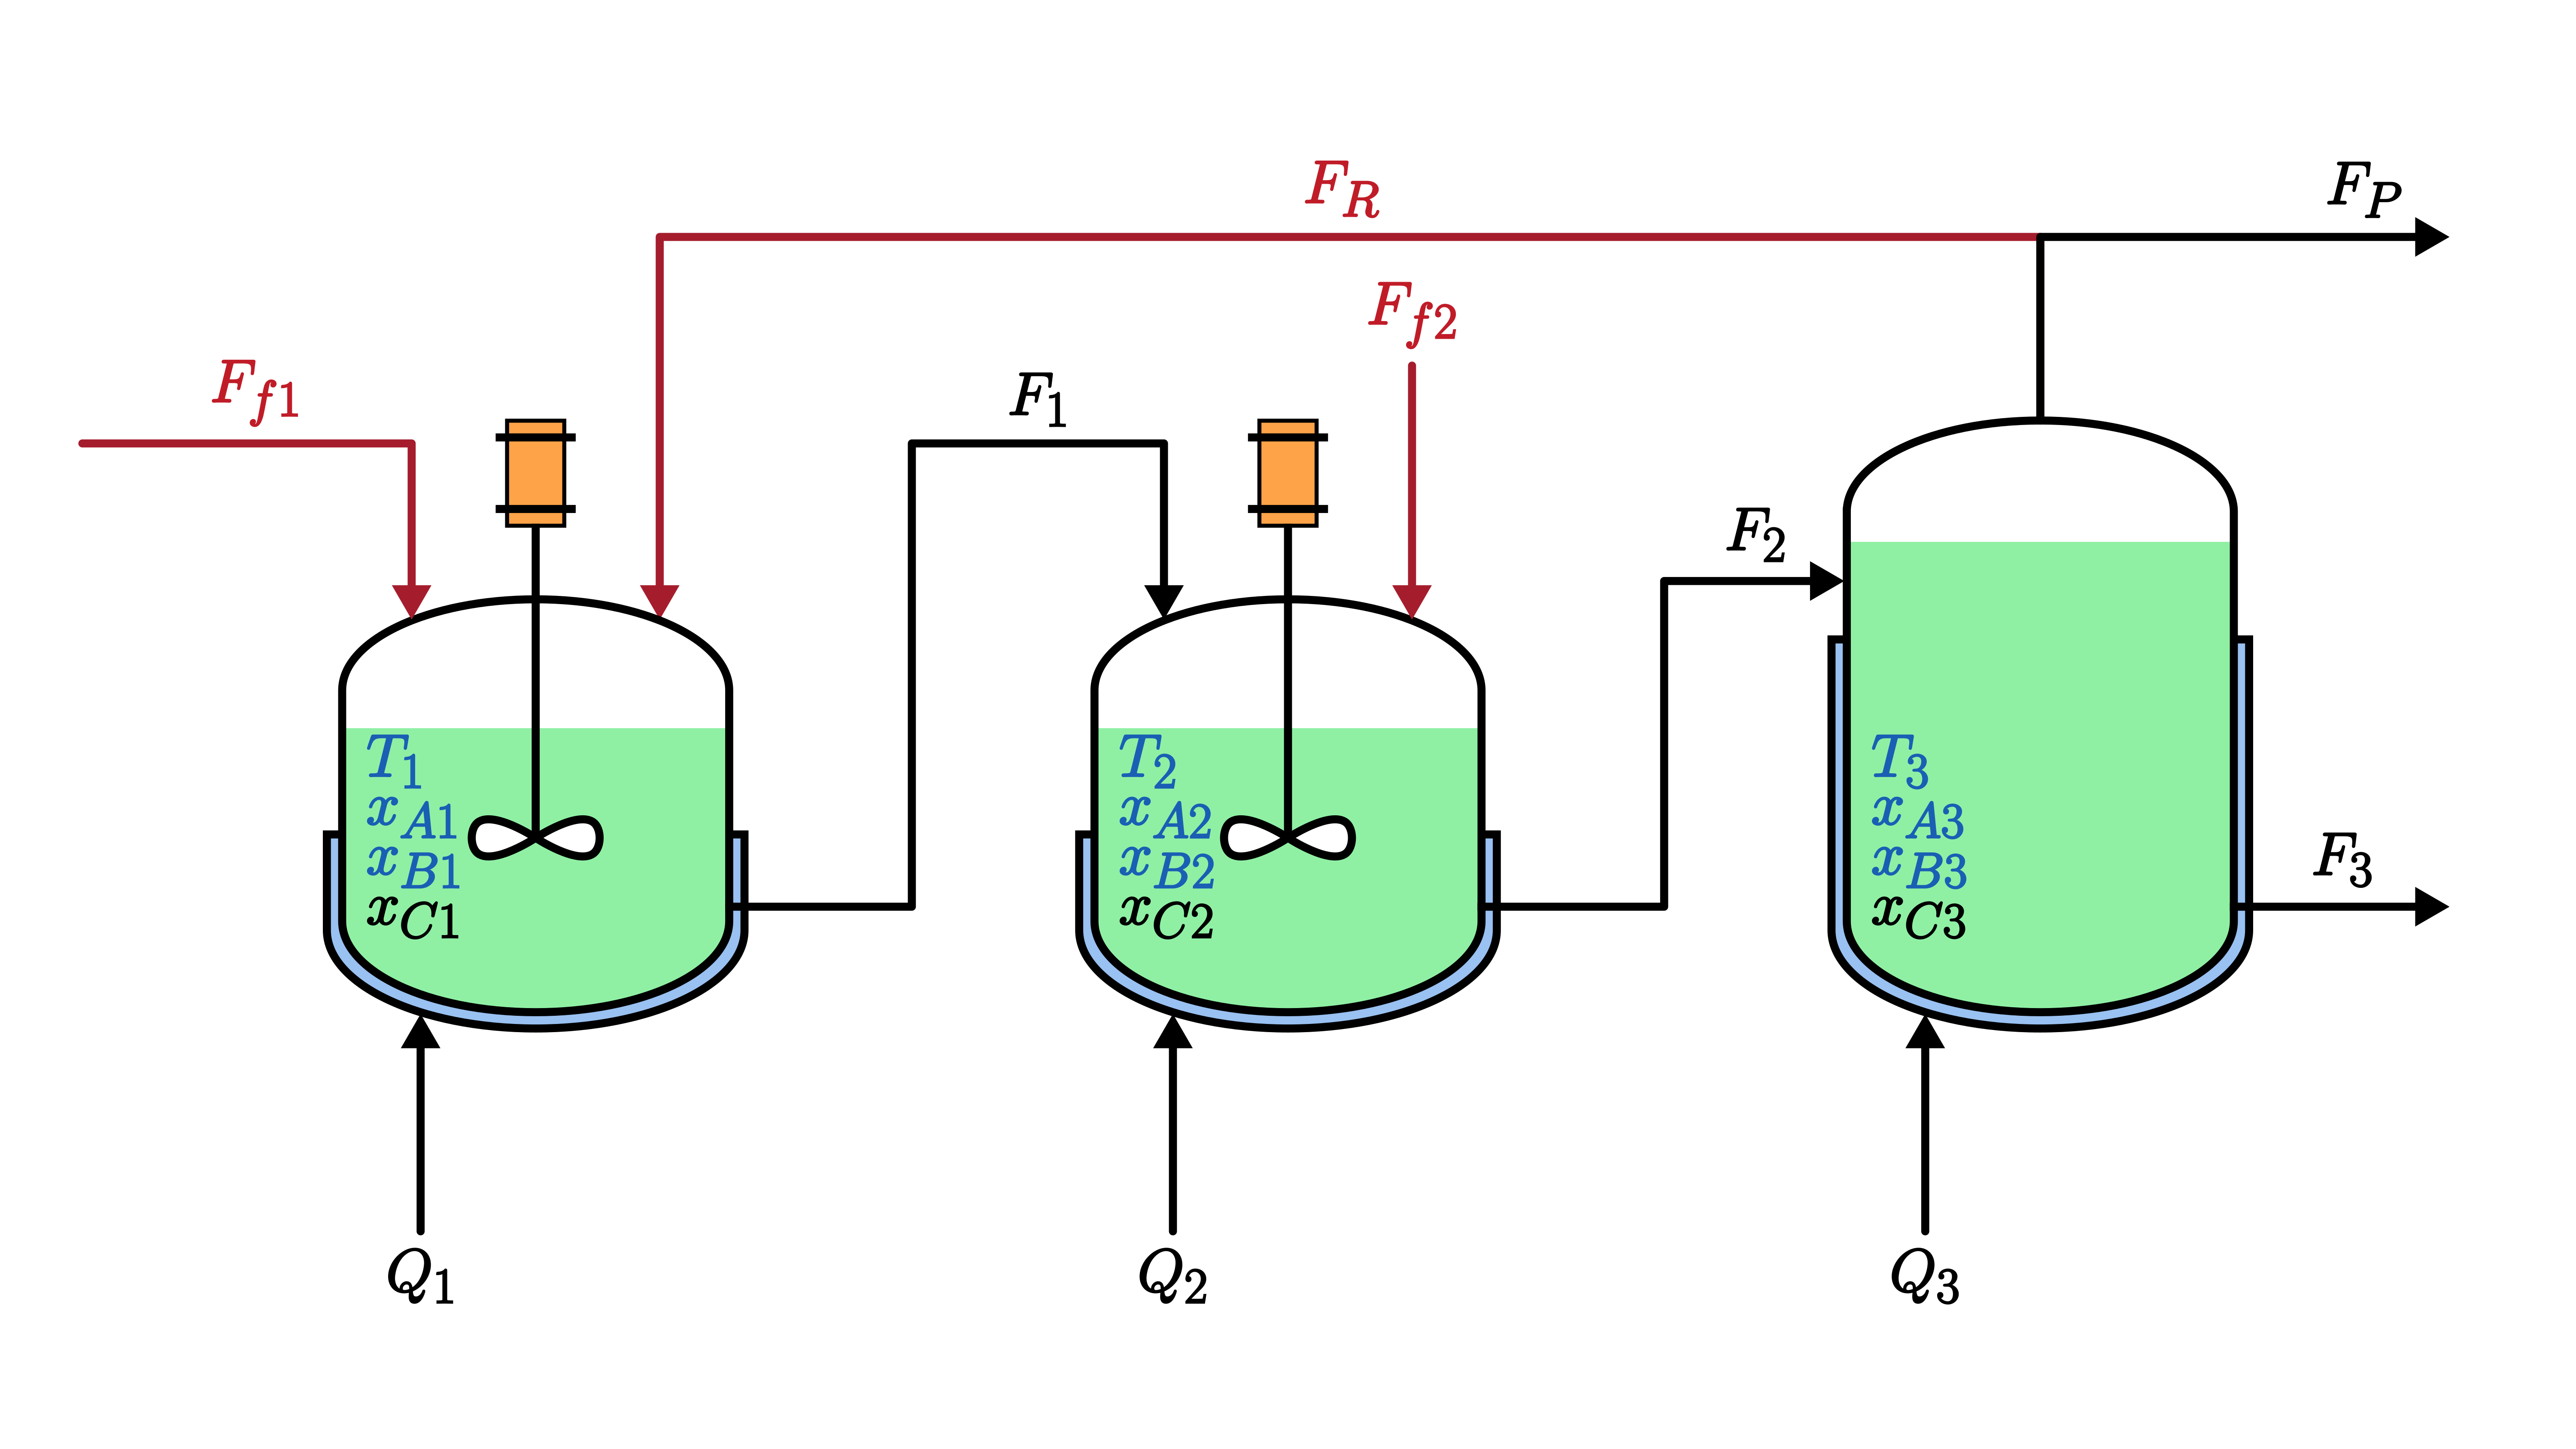
\includegraphics[width=0.6\textwidth]{../../figures/diagram.png}
  \caption{Diagrama do sistema integrado reator-separador utilizado neste trabalho.}
  \label{fig:diagram}
\end{figure}

As entradas do sistema são as vazões de alimentação $F_{f1}$ e $F_{f2}$ e a vazão de reciclo $F_R$, destacadas em vermelho na Figura~\ref{fig:diagram}.
As taxas de calor $Q_i$ e a temperatura de alimentação $T_0$ são mantidas constantes nos valores nominais.
As saídas são os estados de temperatura $T_i$ e de fração molar $x_{Ai}$ e $x_{Bi}$, em que $i = 1, 2, 3$ indica o primeiro reator, o segundo reator e o separador, respectivamente.

A dinâmica é descrita por equações diferenciais não lineares obtidas de balanços de massa e energia, com coeficientes de velocidade de reação dados pela lei de Arrhenius.
O modelo completo e os parâmetros, extraídos de \textcite{pourkargar_2017}, são apresentados no Apêndice~\ref{sec:apendice_modelo}.

Como os volumes $V_i$ têm comportamento integrador, assume-se volume constante, e as vazões internas passam a ser relações algébricas:
\begin{align}
  F_1 & = F_{f1} + F_R    \\
  F_2 & = F_{f2} + F_1    \\
  F_3 & = F_2 - F_P - F_R
\end{align}
com $F_P = \varepsilon F_R$.
Obtém-se assim um modelo MIMO com três entradas e nove estados, tomados como saídas.
